\documentclass[a4paper,man,natbib]{apa6}


\usepackage[english]{babel}
\usepackage[utf8x]{inputenc}
\usepackage{amsthm}
\usepackage{amsmath}
\usepackage{amssymb}
\usepackage{mathtools}
\usepackage{graphicx}
\usepackage[colorinlistoftodos]{todonotes}
\usepackage{url}
\usepackage{xcolor}


\newcommand{\C}{\mathbb{C}}  % Complex
\newcommand{\R}{\mathbb{R}}  % Real
\newcommand{\Z}{\mathbb{Z}}  % Integers
\newcommand{\N}{\mathbb{N}}  % Naturals


\title{Advanced $\C$alculus}
\shorttitle{Written Homework 2}
\author{$\C$ason Konzer}
\date{October, 2021}
\affiliation{University of Michigan}


\begin{document}
\maketitle


\section{\underline{Problem 1}}
\label{sec: Problem 1}

\begin{center}

    Find the Fourier cosine and sine seriers of the even and odd half range expansions of; \\ 

    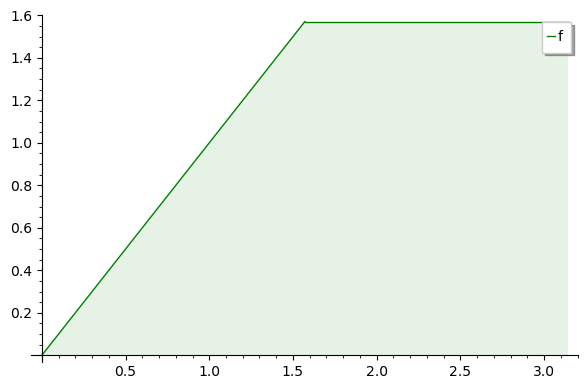
\includegraphics[width=1\textwidth]{C:/Users/user/OneDrive - Umich/Math/Advanced_Calculus/HW/WRITTEN_HW/TEX/HW 2/IMGS/f.png} \\

    \color{teal}
    $ f = \begin{cases}
        x & \quad 0 < x < \frac{\pi}{2} \\
        \frac{\pi}{2} &  \quad \frac{\pi}{2} < x < \pi
    \end{cases}$ \\
    \color{black}

    \hfill \break
    \underline{Euler's Formulas} \\

    \color{purple} $ a_0 $ \color{black} $ = \frac{1}{L}  \int_{0}^{L} f(x) \,dx $ \\

    \color{blue} $ a_n $ \color{black} $ = \frac{2}{L}  \int_{0}^{L} f(x) \cos(\frac{n\pi x}{L}) \,dx $ \\

    \color{red} $ b_n $ \color{black} $ = \frac{2}{L}  \int_{0}^{L} f(x) \sin(\frac{n\pi x}{L}) \,dx $ \\

    \hfill \break
    \underline{Period} \\

    $ p = 2\pi $ ; $ L = p/2 $ ; $ L = 2\frac{\pi}{2} $ ; $ L = \pi $ \\ 

    \underline{Fourier Series} \\

    $ f(x) = a_0 + \sum_{n = 1}^{\infty} a_n \cos(n\pi x/L) + b_n \sin (n\pi x/L) $ \\
    $ f(x) = a_0 + \sum_{n = 1}^{\infty} a_n \cos(nx) + b_n \sin (nx) $ \\


\end{center}


\newpage
\section{\underline{Even Expansion}}
\label{sec: Even Expansion}

\begin{center}

    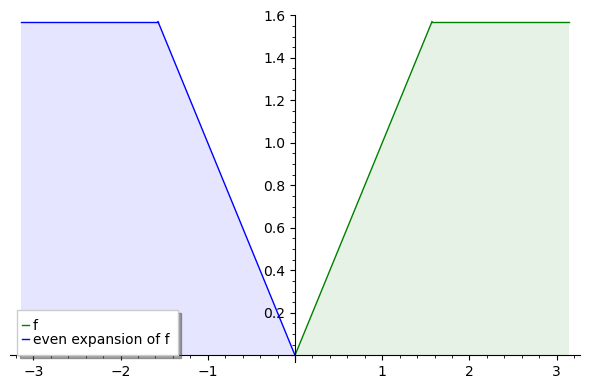
\includegraphics[width=1\textwidth]{C:/Users/user/OneDrive - Umich/Math/Advanced_Calculus/HW/WRITTEN_HW/TEX/HW 2/IMGS/even_expansion_of_f.png} \\
    
    \hfill \break
    $ a_0 = \frac{1}{\pi} \int_{0}^{\pi} f(x) \,dx = \frac{1}{\pi} [\int_{0}^{\pi} x \,dx + \int_{\frac{\pi}{2}}^{\pi} \frac{\pi}{2} \,dx ] $ \\
    $ a_0 = \frac{1}{\pi} [[\frac{x^2}{2} \Big|_{0}^{\frac{\pi}{2}}] + [\frac{\pi x}{2} \Big|_{\frac{\pi}{2}}^{\pi}]] = \frac{1}{\pi} [[\frac{\pi^2}{8}] + [\frac{\pi^2}{2} - \frac{\pi^2}{4}]] 
    = \frac{1}{\pi} [\frac{\pi^2}{8} + \frac{4\pi^2}{8} - \frac{2\pi^2}{8}] $ \\
    \color{violet} $ a_0 = $ \color{black} $ [\frac{\pi}{8} + \frac{4\pi}{8} - \frac{2\pi}{8}] $ \color{violet} $ = \frac{3\pi}{8} $ \color{black} \\
    
    \hfill \break
    $ a_n = \frac{2}{\pi} \int_{0}^{\pi} f(x) \cos(\frac{n\pi x}{\pi}) \,dx  =
    \frac{2}{\pi} \int_{0}^{\pi} f(x) \cos(nx) \,dx $  \\
    $ a_n = \frac{2}{\pi} \int_{0}^{\frac{\pi}{2}} x \cos(nx) \,dx + \frac{2}{\pi} \int_{\frac{\pi}{2}}^{\pi} \frac{\pi}{2} \cos(nx) \,dx $ \\
    $ a_n = \frac{2}{\pi} [\frac{x\sin(nx)}{n} \Big|_{0}^{\frac{\pi}{2}} - \int_{0}^{\frac{\pi}{2}} \frac{\sin(nx)}{n} \,dx] + \int_{\frac{\pi}{2}}^{\pi} \cos(nx) \,dx $ \\
    $ a_n = \frac{2}{\pi} [\frac{\pi\sin(\frac{n\pi}{2})}{2n} - [\frac{-\cos(nx)}{n^2} \Big|_{0}^{\frac{\pi}{2}}]] + [\frac{sin(nx)}{n} \Big|_{\frac{\pi}{2}}^{\pi}] $ \\
    $ a_n = \frac{2}{\pi} [\frac{\pi\sin(\frac{n\pi}{2})}{2n} - [\frac{-\cos(\frac{n\pi}{2})}{n^2} + \frac{1}{n^2}]] + [\frac{sin(n\pi)}{n} - \frac{sin(\frac{n\pi}{2})}{n}] $ \\
    
    $ note: \sin(n\pi) = 0 $ ; $ \forall n \in \N $ 
    $ a_n = \frac{2}{\pi} [\frac{\pi\sin(\frac{n\pi}{2})}{2n} + \frac{\cos(\frac{n\pi}{2})}{n^2} - \frac{1}{n^2}] - [\frac{sin(\frac{n\pi}{2})}{n}] = [\frac{2n\pi\sin(\frac{n\pi}{2})}{2n^2\pi} + \frac{2\cos(\frac{n\pi}{2})}{n^2\pi}- \frac{2}{n^2\pi}] - [\frac{sin(\frac{n\pi}{2})}{n}] $ \\
    \color{blue} $ a_n = $ \color{black} $ [\frac{n\pi\sin(\frac{n\pi}{2}) + 2\cos(\frac{n\pi}{2}) - 2}{n^2\pi}] - [\frac{n\pi\sin(\frac{n\pi}{2})}{n^2\pi}] $ \color{blue} $ = \frac{2\cos(\frac{n\pi}{2}) - 2}{n^2\pi} $ \color{black} \\

    $ note: \cos(\frac{n\pi}{2}) = 0 $ ; $ \forall n \in \{ 1, 3, 5 \dots \} $, \\
    $ \cos(\frac{n\pi}{2}) = -1 $ ; $ \forall n \in \{ 2, 6, 10 \dots \} $, $ \cos(\frac{n\pi}{2}) = 1 $ ; $ \forall n \in \{ 4, 8, 12 \dots \} $
    
    \color{blue}
    $ a_n = \begin{cases}
        -\frac{2}{n^2\pi} & \quad n = 1, 3, 5 \dots \\
        -\frac{4}{n^2\pi} & \quad n = 2, 6, 10 \dots \\
        0 & \quad n = 4, 8, 12 \dots
    \end{cases}$ \\
    \color{black}

    \hfill \break
    \underline{Cosine Fourier Series} \\

    $ f(x) = $ \color{violet} $ \frac{3\pi}{8} $ \color{blue} $ - \sum_{n = 1, 3, 5 \dots}^{\infty} \frac{2}{n^2\pi} \cos(nx) - \sum_{n = 2, 6, 10 \dots}^{\infty} \frac{4}{n^2\pi} \cos(nx) $ \color{black} \\

    $ f(x) = $ \color{violet} $ \frac{3\pi}{8} $ \color{blue} $ -[\frac{2\cos(x)}{\pi} + \frac{4\cos(2x)}{4\pi} + \frac{2\cos(3x)}{9\pi} + \frac{2\cos(5x)}{25\pi} + \frac{4\cos(6x)}{36\pi} \dots] $ \\

    \hfill \break
    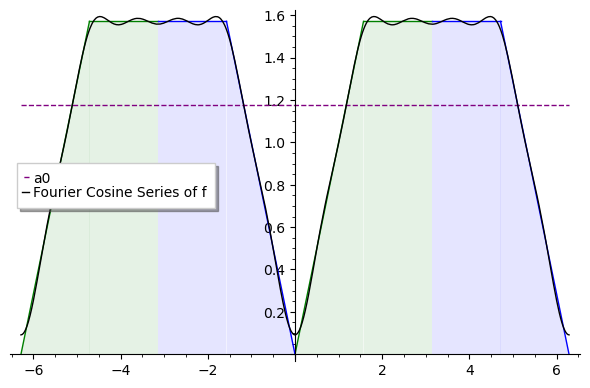
\includegraphics[width=1\textwidth]{C:/Users/user/OneDrive - Umich/Math/Advanced_Calculus/HW/WRITTEN_HW/TEX/HW 2/IMGS/cosine_series_of_f.png} \\

\end{center}

\newpage
\section{\underline{Odd Expansion}}
\label{sec: Odd Expansion}
\begin{center} 

    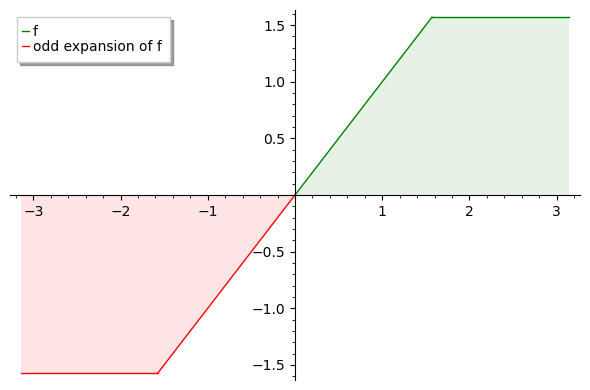
\includegraphics[width=1\textwidth]{C:/Users/user/OneDrive - Umich/Math/Advanced_Calculus/HW/WRITTEN_HW/TEX/HW 2/IMGS/odd_expansion_of_f.png} \\
   
    \hfill \break
    $ b_n = \frac{2}{\pi}  \int_{0}^{\pi} f(x) \sin(\frac{n\pi x}{\pi}) \,dx  =
    \frac{2}{\pi}  \int_{0}^{\pi} f(x) \sin(nx) \,dx $ \\ 
    $ b_n = \frac{2}{\pi}  \int_{0}^{\frac{\pi}{2}} x \sin(nx) \,dx + \frac{2}{\pi}  \int_{\frac{\pi}{2}}^{\pi} \frac{\pi}{2} \sin(nx) \,dx $ \\
    $ b_n = \frac{2}{\pi} [\frac{-x\cos(nx)}{n} \Big|_{0}^{\frac{\pi}{2}} - \int_{0}^{\frac{\pi}{2}} \frac{-\cos(nx)}{n}] + \int_{\frac{\pi}{2}}^{\pi} \sin(nx) \,dx $ \\
    $ b_n = \frac{2}{\pi} [[\frac{-\pi\cos(\frac{n\pi}{2})}{2n}] - [\frac{-\sin(nx)}{n^2} \Big|_{0}^{\frac{\pi}{2}}]] + [\frac{-\cos(nx)}{n} \Big|_{\frac{\pi}{2}}^{\pi}] $ \\
    $ b_n = \frac{2}{\pi} [[\frac{-\pi\cos(\frac{n\pi}{2})}{2n}] - [\frac{-\sin(\frac{n\pi}{2})}{n^2}]] + [\frac{-\cos(n\pi)}{n} - \frac{-\cos(\frac{n\pi}{2})}{n}] $ \\
    
 $ b_n = [\frac{-2\pi\cos(\frac{n\pi}{2})}{2n\pi} + \frac{2\sin(\frac{n\pi}{2})}{n^2\pi}] + [\frac{-\cos(n\pi)}{n} + \frac{\cos(\frac{n\pi}{2})}{n}] $ 
    $ b_n = [\frac{-n\pi\cos(\frac{n\pi}{2})}{n^2\pi} + \frac{2\sin(\frac{n\pi}{2})}{n^2\pi} + \frac{-n\pi\cos(n\pi)}{n^2\pi} + \frac{n\pi\cos(\frac{n\pi}{2})}{n^2\pi}] $ \\
    \color{red} $ b_n = $ \color{black} $ [\frac{2\sin(\frac{n\pi}{2}) + n\pi\cos(\frac{n\pi}{2}) - n\pi\cos(\frac{n\pi}{2}) - n\pi\cos(n\pi)}{n^2\pi}] $ \color{red} $ = \frac{2\sin(\frac{n\pi}{2}) - n\pi\cos(n\pi)}{n^2\pi} $ \color{black} \\

    
    $ note: \sin(\frac{n\pi}{2}) = 1 $ ; $ \forall n \in \{1, 5, 9 \dots \} $, $ \sin(\frac{n\pi}{2}) = -1 $ ; $ \forall n \in \{3, 7, 11 \dots \} $, \\
    $ \cos(n\pi) = -1 $ ; $ \forall n \in \{1, 3, 5 \dots \} $, $ \cos(n\pi) = 1 $ $\&$ $ \sin(\frac{n\pi}{2}) = 0 $; $ \forall n \in \{2, 4, 6 \dots \} $ \\
    
    \color{red}
    \hfill \break
    $ b_n = \begin{cases}
        \frac{n\pi + 2}{n^2\pi} & \quad n = 1, 5, 9 \dots \\
        -\frac{1}{n} & \quad n = 2, 4, 6 \dots \\
        \frac{n\pi - 2}{n^2\pi} & \quad n = 3, 7, 11 \dots
    \end{cases}$ \\
    \color{black}

    \newpage

    \hfill \break
    \underline{Sine Fourier Series} \\

    $ f(x) = $ \color{red} $ \sum_{n = 1, 5, 9 \dots}^{\infty} \frac{n\pi + 2}{n^2\pi} \sin (nx) - \sum_{n = 2, 4, 6 \dots}^{\infty} \frac{1}{n} \sin (nx) + \sum_{n = 3, 7, 11 \dots}^{\infty} \frac{n\pi - 2}{n^2\pi} \sin (nx) $ \color{black} \\ 

    $ f(x) = $ \color{red} $ \frac{(\pi + 2)\sin(x)}{\pi} - \frac{\sin(2x)}{2} + \frac{(3\pi - 2)\sin(3x)}{9\pi} - \frac{\sin(4x)}{4} + \frac{(5\pi + 2)\sin(5x)}{25\pi} - \frac{sin(6x)}{6} + \frac{(7\pi - 2)\sin(7x)}{49\pi} \dots $ \color{black} \\
    
    \hfill \break
    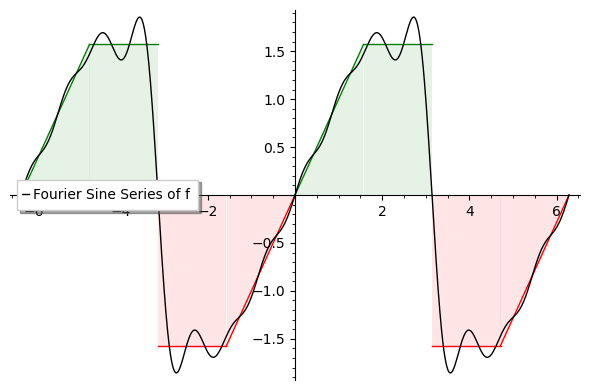
\includegraphics[width=1\textwidth]{C:/Users/user/OneDrive - Umich/Math/Advanced_Calculus/HW/WRITTEN_HW/TEX/HW 2/IMGS/sine_series_of_f.png} \\

    \newpage
    \underline{Average of Fourier Cosine and Sine Series} \\

    \color{teal} $ a(x) = $ \color{black} $ [ $ \color{violet} $ \frac{3\pi}{8} $ \color{blue} $ - \sum_{n = 1, 3, 5 \dots}^{\infty} \frac{2}{n^2\pi} \cos(nx)\ - \sum_{n = 2, 6, 10 \dots}^{\infty} \frac{4}{n^2\pi} \cos(nx) $ \color{red} 
    $ + \sum_{n = 1, 5, 9 \dots}^{\infty} \frac{n\pi + 2}{n^2\pi} \sin (nx) - \sum_{n = 2, 4, 6 \dots}^{\infty} \frac{1}{n} \sin (nx) + \sum_{n = 3, 7, 11 \dots}^{\infty} \frac{n\pi - 2}{n^2\pi} \sin (nx) $ \color{black} $ ]/2 $ \\ 

    \hfill \break
    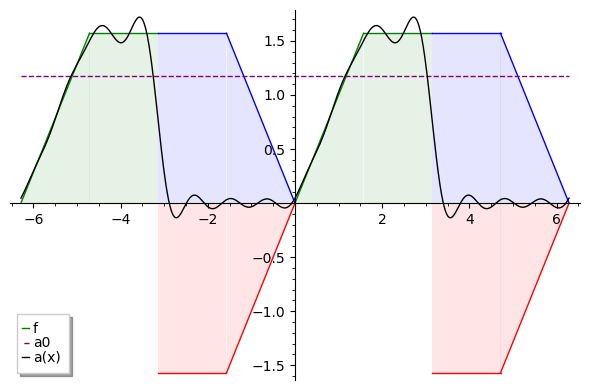
\includegraphics[width=1\textwidth]{C:/Users/user/OneDrive - Umich/Math/Advanced_Calculus/HW/WRITTEN_HW/TEX/HW 2/IMGS/Average.png} \\

\end{center}


\end{document}

%Comments - October 2021 Advanced Calculus Written Home Work #2%